\documentclass[a4paper,12pt]{report}
\usepackage[a4paper,inner = 1.7cm, outer = 2.7cm, top = 2cm, bottom = 2cm, bindingoffset = 1.2cm]{geometry}

\usepackage[romanian]{babel}
\usepackage{blindtext}
\usepackage{fancyhdr}
\usepackage{wrapfig}
\usepackage{graphicx}
\usepackage{amsmath}

\fancyhf{}
\renewcommand{\headrulewidth}{2pt}
\renewcommand{\footrulewidth}{1pt}
\fancyhead[LE]{\leftmark}
\fancyhead[RO]{\rightmark}
\linespread{1.25}
\hyphenpenalty=5000
\begin{document}
\begin{center}
\pagestyle{empty}
       \vspace*{1cm}

       \textbf{UNIVERSITATEA DIN BUCUREȘTI
FACULTATEA DE MATEMATICĂ ȘI INFORMATICĂ}

       \vspace{0.5cm}
        LUCRARE DE LICENȚĂ
            
       \vfill
           
       \vspace{0.8cm}
\textbf{Coordonator:}
\hfill
\textbf{Absolvent:} \\
\textbf{Prof. Dr. Radu Ionescu}
\hfill
\textbf{Moldovan George-Alexandru} \\

\vspace{0.8cm}
      București \\
Iunie (fingers crossed), 2020
\clearpage         
\end{center}
\newpage

\begin{center}
\pagestyle{empty}
       \vspace*{1cm}

       \textbf{UNIVERSITATEA DIN BUCUREȘTI
FACULTATEA DE MATEMATICĂ ȘI INFORMATICĂ}

       \vspace{0.5cm}
        Sistem pentru detectarea anomaliilor in video
            
       \vfill
           
       \vspace{0.8cm}
\textbf{Coordonator:}
\hfill
\textbf{Absolvent:} \\
\textbf{Prof. Dr. Radu Ionescu}
\hfill
\textbf{Moldovan George-Alexandru} \\
    
\vspace{0.8cm}  
	București \\
Iunie (fingers crossed), 2020
\clearpage
\end{center}
\newpage

\tableofcontents
\listoffigures
\pagenumbering{arabic}
\setcounter{page}{2}
\begin{abstract}
\par Având în vedere contextul actual, detectarea anomaliilor în video este un subiect de interes în mai multe arii, în mod special în securitatea publică. Putem spune că această problemă este încă nerezolvată, deoarece sistemele actuale, deocamdată, nu depăşesc  omul cand vine vorba de detectarea anomaliilor. De asemenea, o altă problemă a sistemelor de detectare a anomaliilor în video este nevoia acestora de resurse computaţionale mari în partea de inferență, făcând aproape imposibilă rularea acestora direct pe hardware-ul existent al sistemelor de supraveghere video actuale, acolo unde acestea prezintă un maxim interes. Astfel, putem spune că dezvoltarea unui sistem capabil să transforme sistemele de supraveghere actuale în sisteme ce pot recunoaşte evenimente anormale  este un subiect ce poate revoluţiona domeniul supravegherii video. Această lucrare îşi propune o implementare al sistemului state-of-the-art la momentul redactării, aşa cum este prezentat de \emph{Ionescu et al.} \cite{ionescu2019object}. Obiectivul este obţinerea unei arhitecturi ce foloseşte o soluţie PaaS si expunerea etapei de inferenţă printr-un API astfel încât convertirea unui sistem de supraveghere clasic într-unul inteligent să devină doar o problemă de implementare, fără a fi nevoie de schimbarea hardware-ului. Utilizarea unei soluţii PaaS pentru etapa de inferenţă rezolvă problema executării cererilor fără complexitatea creeri şi întreţinerii unei infrastructuri de maşini virtuale sau fizice. 
\end{abstract}

\chapter{Introducere}
\section{Motivatie}
\quad Detectarea anomaliilor în video este în strânsă legătură cu sistemele de supraveghere inteligente,un domeniu care a fost şi este de interes pentru mine. La rândul lor, sistemele de supraveghere inteligente, au o mare importanţă în securitatea publică. Cu toţii ne dorim o lume în care apelurile de urgenţă în caz de incendiu se fac automat, alunecările de teren sunt descoperite înainte să fie prea târziu, iar oamenii rău intenţionaţi sunt opriţi înainte să se întâmple tragedii. 
\par
Astfel, arhitectura folosită se bazează pe detecţia caracteristicilor spaţio-temporale ale evenimentelor prezente în video, care mai apoi sunt împărţite în clase de normalitate. Aceste caracteristici sunt extrase trecând evenimentul printr-o serie de autoencodere pentru a folosi mai apoi reprezentarea latentă în cadrul clasificării finale. În etapa de antrenare, se folosesc filmări ce prezintă comportamentul normal în scenariul analizat. Analizând aceste video-uri putem creea un model capabil să recunoască dacă un eveniment aparţine unei clase de normalitate analizate până acum, sau dacă este un caz anormal. Deoarece un eveniment poate fi ales în multe moduri, în cadrul acestui sistem un eveniment reprezintă orice obiect aflat în cadru. Analiza asupra fiecarui obiect conţine şi un cadru precedent dar si unul viitor, asemănător cu modalitatea folosită de \emph{Ionescu et al.}  \cite{ionescu2019object}. O menţiune în acest sens ar fi că  pentru fiecare obiect sunt analizate si cadrele de la poziţiile t-3 si t+3  respectiv la poziţia t a cadrului analizat. Din acest motiv, atunci când sistemul va analiza un video în sistem live-feed, analiza se va face cu un decalaj de 3 cadre. Având în vedere că pentru un video actual viteza de redare este de minim 15 cadre pe secundă, acest decalaj este neglijabil.
\par
Pe lângă partea algoritmică a detectării anomaliilor, o altă arie de interes a acestei lucrări este cloud computing. Această parte analizează un nou mod de rulare, ce facilitează atât dezvoltarea cât şi execuţia ulterioară a unor sisteme complexe. Acest nou mod constă în folosirea unei arhitecturi plasată în cloud, ce oferă dezvoltatorului posibilitatea să creeze sisteme ce necesită multe resurse în timpul rulării, fără costurile asociate creeri şi menţinerii unei infrastructuri proprii. Pe de altă parte, având în vedere că toate operaţiunile sunt executate in cloud, utilizatorii serviciului au nevoie doar de conexiune la internet şi cerinţe minime pentru sistemele proprii, fara a fi nevoiţi să achiziţioneze echipamente noi pentru a folosi sisteme de detecţie a anomaliilor.
\section{Context}
\quad Detectarea anomaliilor în video poate fi văzută ca o problemă subiectivă, deoarece un eveniment este normal sau anormal doar dacă este luat în considerare şi contextul în care acesta apare. Un exemplu foarte bun este comparaţia între două persoane care se luptă şi o persoană care se plimbă. Care dintre aceste evenimente este anormal ? Desigur, depinde de context. Dacă sistemul supraveghează o arenă de lupte, atunci persoana care se plimbă în ring prezintă un comportament anormal, în timp ce luptătorii prezintă comportamentul aşteptat. Din acest motiv majoritatea lucrărilor din domeniu \cite{cheng2015,ionescu2019object,sultani2018}...  abordează un mod de lucru bazat pe antrenarea folosind video-uri ce provin din aceeasi locaţie cu cele de test. Tocmai din cauza dependenţei de context, detectarea anomaliilor nu este o problemă ce poate fi generalizată, astfel fiecare scenariu necesită o antrenare şi un model propriu. \par

Ca şi moduri de expunere a soluţiei software către utilizatori, aceasta se poate face în 2 moduri :
\begin{itemize}
\item Folosind servere proprii
\item Folosind servicii cloud
\end{itemize}
\par

\begin{wrapfigure}{r}{0.45\textwidth}
	  \begin{center}
        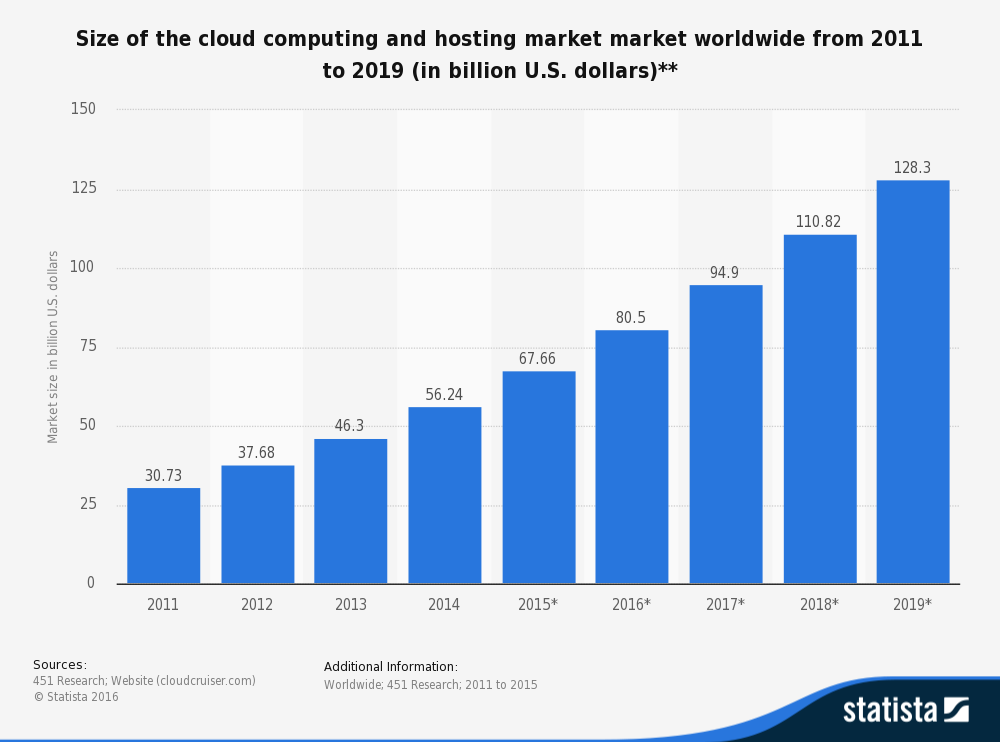
\includegraphics[width=0.4\textwidth]{images/grafic_cloud_computing}
			\label{fig:cloud_computing_graph}
       \caption{Statistică ce evidenţiază importanţa domeniului cloud computing în ultimii ani}
    \end{center}
\end{wrapfigure}

Folosirea serverelor proprii presupune, pe lângă prezenţa fizică a serverelor şi cumpărarea tuturor serviciilor conexe, cum ar fi servere de baze de date, sisteme de distribuire a fişierelor, infrastructură de reţea, ş.a.m.d., este nevoie si de o echipă dedicată pentru întreţinerea infrastructurii şi repararea eventualelor probleme ce pot apărea. Aceste considerente, împreuna cu faptul că scalarea soluţiilor software este foarte anevoioasă atunci când este folosită infrastructura proprie, fac această soluţie să nu mai fie folosită în mod curent deoarece incetineşte dezvoltarea aplicaţiei, iar rezultatul final este şi el unul mai puţin calitativ decât ce se poate obţine folosind soluţii în cloud. 
\par
Folosirea serviciilor cloud oferă multiple posibilităţi de dezvoltare a aplicaţiilor, de la creeare unei infrastructuri complete care este administrată în totalitate de către dezvoltator, la medii de execuţie serverless care sunt complet administrate de către provider-ul de servicii cloud. 
Deşi creearea unei infrastructuri proprii încă este necesară acolo unde legislaţia nu permite ca datele sa fie stocate în cloud, în toate celelalte cazuri se face migrarea spre soluţii cloud, lucru vizibil şi în evoluţia cotei de piaţă a domeniului cloud-computing la nivel global, aşa cum se poate observa şi in figura ~\ref{fig:cloud_computing_graph}. 

\section{Conţinutul lucrării}
 Ca şi structură, lucrarea este împărţită în 2 părţi:
\begin{itemize}
\item Partea algoritmică a sistemului de detectare a anomaliilor în video
\item Partea de deployment a sistemului
\end{itemize}
\par În prima parte sistemul va fi analizat si detaliat din punct de vedere algoritmic si teoretic studiind problema detecţiei propriu zisă. Ca şi tehnologii, in această parte am ales sa folosesc Python3 ca şi limbaj de programare pentru anvantajele pe care le are. Printre acestea se numără faptul ca este un limbaj orientat pe obiecte care pune la dispozitia dezvoltatorului numeroase librării specifice pentru AI/ML mutând astfel atenţia dinspre detalii de implementare spre detalii de arhitectură şi probleme mai abstracte ale programului care sunt cu adevărat importante pentru rezultatul final. Una dintre librăriile care s-a dovedit esenţială dezvoltarii este \emph{Keras} \cite{2020keras}, care oferă un API ce uşurează dezvoltarea unei reţele neuronale adânci/convoluţionale dar şi optimizează timpul de antrenare pentru modelele create.  \par
În cea de a doua parte este analizat tipul de deployment al aplicaţiei. Aici vor fi prezentate analize detaliate ale avantajelor si dezavantajelor soluţiilor cloud, dar si motivele pentru care modul final de deployment a fost ales. \\
Soluţiile de cloud-computing analizate vor fi:
\begin{itemize}
\item Infrastructure as a Service (IaaS) - analiză pe Amazon EC2
\item Platform as a Service (PaaS) - analiză pe Amazon Elastic Beanstalk
\item Function as a Service (FaaS) - analiză pe Amazon Lambda
\end{itemize}
\chapter{Analiza arhitecturii si a tehnologiilor folosite}
\quad Pentru o mai bună înţelegere a contextului în care tehnologiile prezentate au fost folosite, acestea vor fi prezentate mai jos in cadrul secţiunii corespunzătoare locului în care a fost folosită în cadrul proiectului. Pentru toate etapele sistemului, limbajul folosit este Python3, deoarece, împreună cu librariile si framework-urile existente pentru inteligenţă articială, reprezintă mediul ideal pentru dezvoltarea unei soluţii modulare, rapide si uşor de modificat.
\section{Etapa de antrenare}
Pentru etapa de antrenare, sistemul trece prin următoarea serie de etape: 
\begin{itemize}
\item Detectează obiectele din setul de date
\item Antrenează un autoencoder pe imaginile obiectelor si un alt autoencoder pe gradienţii obiectelor.
\item Obţine reprezentarea latentă a fiecărui eveniment
\item Stabileşte k clase de normalitate folosind reprezentările latente
\item Antrenează k clasificatori de tipul one-versus-rest
\end{itemize}
\par Ca prim pas, pentru obţinerea obiectelor dintr-o imagine, atât în etapa de antrenare cât şi în cea de inferenţă este folosit un detector de obiecte pre-antrenat. Un detector de obiecte este un sistem ce primeşte ca input o imagine si după procesarea acesteia rezolvă problema detecţiei de obiecte şi întoarce poziţiile la care sunt plasate obiectele în imagine, şi etichetele asociate acestora. Deşi detectorul de obiecte face parte din arhitectură, deoarece detectarea de obiecte este un subiect în sine, implementarea unui astfel de algoritm nu face obiectul acestei lucrări. Datorită acestui lucru, este folosit un detector deja antrenat din biblioteca \emph{gluoncv} si testat pe setul de date COCO. 
\par După aceasta etapă sunt antrenate cele două autoencodere convoluţionale. Unul pentru imaginea propriu-zisă şi altul pentru gradient. Un autoencoder este un tip de reţea neuronală alcătuit din 2 parţi (encoder si decoder) care este folosit pentru a obţine reprezentarea latentă a unui obiect folosind un mod de învăţare nesupervizată. În timpul antrenării, autoencoder-ele au ca scop modificarea parametrilor interni pentru a obţine la ieşire, datele primite la intrare. Deşi ieşirea unui autoencoder nu prezintă interes, ceea ce este folositor este reprezentarea latentă (rezultatul encoder-ului) a datelor. Folosind această tehnică, se obţine o reducere a dimensionalităţii ce imbunătăţeşte semnificativ performanţele clasificatorilor ulteriori. 
\par Obţinerea reprezentării latente a fiecărui obiect se realizează trecând imaginea, respectiv gradientul său prin encoderul autoencoderului corespunzător si păstrarea rezultatului.
\par Odată obţinut vectorul de caracteristici pentru toate obiectele din setul de date, urmează stabilirea claselor de normalitate. Acest lucru se realizează prin aplicarea algoritmului k-means de clustering. Pentru implementare a fost folosit algoritmul \emph{LLoyd} implementat în biblioteca python \emph{sklearn}. Aplicând acest algoritm peste vectorii de caracteristici obţinuţi, rezultă k categorii de normalitate cu vectorii de caracteristici aferenţi. 
\par Folosind categoriile de normalitate obţinute la pasul anterior, putem spune că faţă de o anumită categorie \emph{i}, celelalte k-1 categorii reprezintă categorii \emph{artificial} anormale. Le numim \emph{artifical} anormale deoarece în mod obiectiv ele sunt acţiuni normale pentru sistemul de dectare a anomaliilor, dar pentru antrenarea unor clasificatori conform schemei one-vs-rest acestea sunt tratate drept anormale. Astfel, putem antrena un clasificator binar g(i) în aşa fel încat să separăm elementele din categoria i de cele din categoriile \{1,2...k\}/i 
generând funcţia : \[f_{i}(x) = \sum_{1}^{n} w_{j} * x_{j} + b\]. Unde x \(\in{R}^n\) reprezintă vectorul de caracteristici, w este vectorul de parametri a funcţiei, iar b reprezintă bias-ul funcţiei. \cite{ionescu2019object}.
\par Astfel, generăm k astfel de funcţii corespunzătoare celor k clasificatori ce vor fi folosiţi pentru a stabili daca un eveniment este anormal. Conform schemei one-vs-rest, un eveniment este anormal daca este clasificat drept anormal de către toţi cei k clasificatori.
\vfill
\section{Etapa de inferenţă}
\quad În cadrul etapei de inferenţă, sistemul foloseşte detectorul de obiecte, autoencoderele pre-antrenate şi cei k clasificatori binari pentru a stabili dacă un anumit eveniment este sau nu anormal. Astfel, parcursul sistemului este următorul :
\begin{itemize}
\item Extragerea cadrelor necesare din video
\item Extragerea obiectelor din imagini
\item Obţinerea reprezentării latente
\item Clasificarea evenimentelor
\end{itemize}
\par
Pentru analiza unui eveniment care apare la un indice dat \emph{t} sunt necesare 3 cadre. Mai precis cadrele de la indicii \emph{t-3}, \emph{t+3} şi \emph{t}.
Din cadrul t se va extrage vectorul de caracteristici specific aparenţei vizuale, iar din celelalte 2 cadre se vor extrage vectorii de caracterisitici specifici mişcării obiectului, prin analiza gradienţilor. Prin concatenarea acestor 3 vectori, se obţine vectorul final de caracteristici ce va fi folosit drept input pentru clasificatorii finali.
\par
Pentru extragerea obiectelor din cadrele analizate, se va folosi acelaşi detector de obiecte ca în etapa de antrenare.  Acesta va fi rulat pe cadrul principal t, urmând apoi sa se folosească coordonatele obiectelor de la cadrul t, si pentru cadrele t+3 si t-3 deoarece din cauza diferenţei mici de indici, obiectele nu se pot mişca indeajuns incât sa fie necesară rularea pe toate cele 3 cadre.
\par
Odată obţinute obiectele din cadrul analizat, dupa obţinerea gradienţilor din cadrele t-3 si t+3, se poate obţine reprezentarea latentă a acestor informaţii.
Reprezentarea latentă a imaginii obiectului constă în rezultatul generat de encoderul autoencoderului pentru imagini iar reprezentarea latentă a gradienţilor constă în rezultatul generat de encoderul autoencoderului pentru gradienţi.
\par
Odată obtinuţi vectorii de caracteristici pentru reprezentarea vizuală şi pentru reprezentarea mişcării obiectului, prin concatenarea lor se obţine vectorul final, ce poate fi folosit drept input pentru clasificarea finală. Conform schemei \emph{one-vs-rest} acest vector este clasificat de toţi cei k clasificatori, iar rezultatul final este scorul maxim obţinut în urma clasificării.
\section{Etapa de deployment}
Pentru a face sistemul public, acesta este lansat drept un API ce rulează etapa de inferenţă pe un server web plasat in cloud. Pentru dezvoltarea serverului am ales să folosesc framework-ul \emph{Flask}. Flask este un micro-framework de python folosit pentru dezvoltarea soluţiilor web. Motivele pentru care acest framework a fost ales sunt : 
\begin{itemize}
\item Acesta adaugă un overhead foarte mic aplicaţiei, lucru esenţial atunci cand aplicaţie se doreşte a fi plasată in cloud, din cauza limitărilor de memorie. 
\item Oferă un suport foarte bun pentru planificarea rutelor de intrare în aplicaţie, lucru foarte important atunci când se doreşte dezvoltarea unui API.
\item Este unul dintre framework-urile suportate de Amazon Elastic Beanstalk 
\end{itemize}
\par
Comparativ cu alte framework-uri, Flask este diferit deoarece nu impune linii clare dezvoltatorilor atunci când vine vorba de forma sau componentele aplicaţiei ce urmează a fi dezvoltată. Astfel, dezvoltatorul are control complet asupra aplicaţiei si îşi poate manifesta creativitatea sau ideile fara a fi restricţionat de framework.  Flask a fost creat tocmai cu ideea de a fi construit peste el. Deşi poate nu oferă aceeaşi viteză de dezvoltare comparativ cu celelalte frameworkuri, acesta oferă libertatea de alegere la fiecare pas. Are suport pentru toate tipurile de baze de date, fie ele relaţionale sau nerelaţionale,  nu are preferinţe când vine vorba de metode de autentificare sau de creare a rolurilor, totul este suportat şi totul este la latitudinea dezvoltatorului. 
\cite{flask2014}
\par
Pentru a lansa serverul in cloud, am folosit serviciul Amazon Elastic Beanstalk. Acesta este un serviciu complex, ce însumează la rândul lui mai multe servicii cloud oferite de Amazon Web Services(AWS). Mai jos sunt prezentate câteva dintre avantajele si dezavantajele acestui serviciu, fiind analizat in detaliu in capitolele ce urmează.  Elastic Beanstalk este un serviciu de tipul \emph{PaaS}  ce ofera servicii de deployment si administrate complete.Pentru o mai bună detaliere, mai jos sunt definite toate serviciile cloud incluse de Elastic Beanstalk: 
\begin{itemize}
\item Amazon EC2 : este un serviciu web oferit de Amazon ce constă în oferirea unui mediu de execuţie sigur in cloud. Este echivalentul unei maşini fizice mutate in cloud. Acesta a fost creat pentru a uşura misiunea dezvoltatorilor de a migra serviciile proprii spre cloud computing.  Aceste instanţe sunt extrem de configurabile, punând la dispoziţia dezvoltatorului mai mult de 50 de tipuri de instanţe, plus diferite opţiuni de optimizare a unor părţi specifice, cum ar fi memoria sau placa video. \cite{2020EC2}
\item Amazon S3 : este un serviciu ce oferă medii de stocare în cloud. Stocarea este de tipul cheie-obiect, unde cheia identifică unic la nivel global un fişier. Acesta oferă o securitate sporită a datelor, şi o disponibilitate de 99.999999\% deoarece datele sunt distribuite în sisteme diferite şi în zone diferite.
\cite{2020S3}
\item Auto Scaling Group : acest serviciu oferă un mod automat de lansare a instanţelor EC2 astfel încât traficul să nu depăşească niciodata puterea de execuţie a unui aplicaţii. Scopul acestui serviciu este de a oferi capacitatea de a scala pentru a menţine o performanţă optimă, menţinând costul în tot acest timp la valoarea minimă.
\cite{2020autoscaling}
\item Elastic Load Balancing: este un serviciu care împarte traficul administrat de aplicaţie către instanţele lansate astfel încât acestea să fie utilizate intr-un. mod optim. Astfel, poate suporta încarcătura variabilă a aplicaţiei şi o poate distribui în aşa fel încat, în funcţie de modul ales(\emph {accesibilitate crescută}, \emph(scalare automată), \emph{securitate ridicată}) aplicaţia să nu scadă sub performanţele dorite.
\cite{2020elb}
\end{itemize}
\par 
\begin{figure}
\begin{center}
        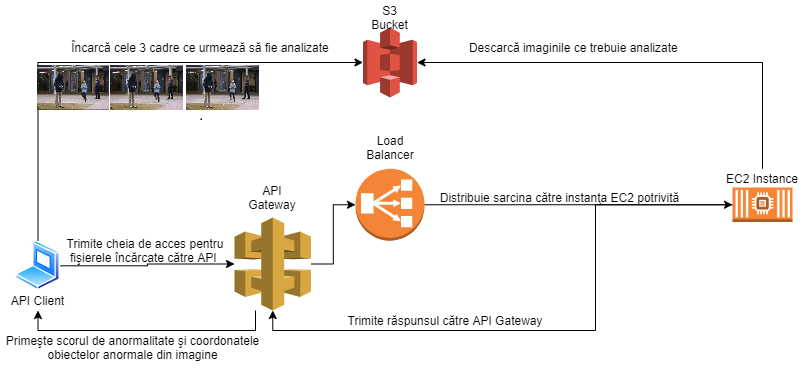
\includegraphics[width=1\textwidth]{images/client_drawing}
			 \label{fig:client_design}
			 \caption{Arhitectura abstractizată a API-ului}
\end{center}
\end{figure}

Dezvoltatorul se ocupă doar de aplicaţia/serverul propriu zis, crează pachetul de deployment, iar Elastic Beanstalk crează instanţele EC2 necesare, administrează si rutează traficul către instanţe folosind un Load Balancer, iar atunci cand aplicaţia este suprasolicitată, lansează în mod automat noi servere folosindu-se de avantajele unui Auto Scaling Group.
\par Aşa cum se poate observa în figura ~\ref{fig:client_design}, API-ul este creat în aşa fel încât evaluarea se face pentru fiecare cadru în parte. Dezvoltatorul ce implementează clientul pentru API are doar responsabilitatea urcării cadrelor necesare într-un spaţiu S3 prestabilit. Preprocesarea, extragerea obiectelor din imagine, şi rularea detecţiei de anomalii sunt toate executate in cloud. Astfel, efortul computaţional asupra clientului este minim. La momentul accesării API-ului, serverul trebuie să primeasca ca parametru în apelul HTTP cheia de acces pentru cadrele urcate de catre client. Folosind această informaţie, pe server se descarcă aceste cadre şi sunt analizate pentru a detecta anomaliile din cadrul central. Ca şi rezultat, clientul primeşte scorul de anormalitate al cadrului împreună cu toate poziţiile obiectelor anormale din cadru, date ce pot fi folosite pentru notificări ulterioare sau diferite aplicaţii pe partea de client. 
\chapter{Plictiseala}
In ceea ce priveşte FaaS, acesta este un domeniu nou, deoarece a apărut pentru prima data in 2010 fiind oferit de câteva start-upuri la acea vreme. Acest mod de dezvoltare orientat spre microservicii a devenit trendul in industrie în ultimii ani pentru sisteme cu potenţial de scalare mare, deoarece prezintă numeroase avantaje din punct de vedere al modului de dezvoltare si de executie in industrie. In momentul de faţă, pentru servicii de tip FaaS sunt 3 mari jucători: Amazon cu AWS Lambda, Google cu Google Cloud Functions si Microsoft cu Azure Functions.\cite{jonas2019cloud}. Numeroase lucrări din domeniu \cite{christidis2019, wang2019} arată ca rularea algoritmilor de machine learning folosind soluţii FaaS (Function as a service) precum AWS Lambda sau Google cloud functions, este în sine o problemă ce necesită soluţii de optimizare a codului pentru a indeplini restricţiile soluţiilor de rulare serverless, cum ar fi memoria limitată a mediului de execuţie. 
\blindtext[3]

\bibliographystyle{abbrv}
\bibliography{References}
\end{document}